\section{Raw Data Quality Control and Agreement Calculation}
\label{app:quality_control_raw}

\subsection{Per‑Annotator Performance vs.\ Expert}

Table~\ref{tab:raw_annotator} reports the number of images on which each annotator agreed with the independent expert.

\begin{table}[htbp]
\centering
\caption{Individual annotator agreement with the expert on the 279‑image review set.}
\label{tab:raw_annotator}
\small
\setlength{\tabcolsep}{6pt}
\begin{tabular}{l c c c}
\toprule
\textbf{Annotator} & \textbf{Correct} & \textbf{Incorrect} & \textbf{Accuracy} \\
\midrule
Annotator 1 & 236 & 43 & 0.846 \\
Annotator 2 & 235 & 44 & 0.842 \\
Annotator 3 & 236 & 43 & 0.846 \\
\bottomrule
\end{tabular}
\end{table}

On average, an individual annotator agreed with the expert on roughly 84.5\% of the images.

\subsection{Consensus (Majority Vote) vs.\ Expert}

The final label for each image was obtained by majority voting among the three annotators. Table~\ref{tab:conf_matrix} shows the confusion matrix between this consensus label and the expert label.

\begin{table}[htbp]
\centering
\caption{Confusion matrix, consensus (majority vote) vs.\ expert on the 279‑image review set.}
\label{tab:conf_matrix}
\small
\setlength{\tabcolsep}{3pt}
\begin{tabular}{l c c c c c c | c}
\toprule
 & \texttt{binhthuong} & \texttt{chaymepla} & \texttt{domla} & \texttt{gisat} & \texttt{moctrang} & \texttt{repsap} & \textbf{Total} \\
\midrule
\texttt{binhthuong} & 43 & 1 & 1 & 1 & 0 & 0 & 46 \\
\texttt{chaymepla}  &  1 & 43 & 1 & 0 & 1 & 0 & 46 \\
\texttt{domla}      &  1 & 1 & 43 & 0 & 0 & 1 & 46 \\
\texttt{gisat}      &  1 & 0 & 0 & 44 & 1 & 1 & 47 \\
\texttt{moctrang}   &  0 & 1 & 0 & 1 & 44 & 1 & 47 \\
\texttt{repsap}     &  0 & 0 & 1 & 1 & 1 & 44 & 47 \\
\midrule
\textbf{Total}      & 46 & 46 & 46 & 47 & 47 & 47 & 279 \\
\bottomrule
\end{tabular}
\end{table}

\subsection{Calculation of Agreement Metrics}

From the confusion matrix:

\begin{itemize}
    \item[a.] \textbf{Observed agreement} ($p_o$) = sum of diagonal elements / total images = $(43+43+43+44+44+44) / 279 = 261 / 279 \approx 0.9355$, reported as $0.94$.
    \item[b.] \textbf{Expected agreement by chance} ($p_e$) is computed from the marginal distributions. Row totals $R$ and column totals $C$ are identical, both equal to $(46,46,46,47,47,47)$. Hence
    \begin{equation}
        p_e = \frac{\sum_{i=1}^{6} R_i \, C_i}{N^2} = \frac{3 \times 46^2 + 3 \times 47^2}{279^2} = \frac{3 \times 2116 + 3 \times 2209}{77841} = \frac{12975}{77841} \approx 0.1667.
    \end{equation}
    \item[c.] \textbf{Cohen's Kappa} is then
    \begin{equation}
        \kappa = \frac{p_o - p_e}{1 - p_e} = \frac{0.9355 - 0.1667}{1 - 0.1667} = \frac{0.7688}{0.8333} \approx 0.9226,
    \end{equation}
    which is rounded to $0.92$ in the main text.
\end{itemize}

These results confirm that the three‑annotator consensus achieves very high agreement with the expert ($93.5\%$ observed agreement, $\kappa = 0.92$), validating the annotation protocol.










\section{Extended Difficulty Analysis}
\label{app:difficulty}

This appendix provides supplementary details for the difficulty analysis presented in Section~\ref{sec:dataset_analysis}, Section~\ref{subsec:difficulty}.

\subsection{Software and Implementation Details}

All experiments were implemented in Python 3.10 using PyTorch 2.0.0 for feature extraction. The t-SNE projection was performed using the scikit-learn implementation with perplexity 30, 1000 iterations, and a random state of 42. Logistic regression was implemented via scikit-learn's \texttt{LogisticRegression} with the LBFGS solver and a maximum of 1000 iterations to ensure convergence.

\subsection{Mathematical Definition of Metrics}

For completeness, we restate the three clustering evaluation metrics used in the main paper.

\paragraph{Silhouette Score}
For a sample \(i\) assigned to cluster \(C_I\), let \(a(i)\) be the mean distance between \(i\) and all other points in the same cluster, and \(b(i)\) the mean distance between \(i\) and all points in the nearest neighbouring cluster. The Silhouette score of \(i\) is:
\[
s(i) = \frac{b(i) - a(i)}{\max\{a(i), b(i)\}}.
\]
The overall Silhouette score is the average of \(s(i)\) over all samples. The score ranges from \(-1\) (poor clustering) to \(+1\) (excellent clustering). A value near zero indicates substantial overlap between clusters.

\paragraph{Davies–Bouldin Index (DBI)}
For each cluster \(C_i\), define its scatter \(S_i\) as the average distance of points in \(C_i\) to its centroid. For two clusters \(C_i\) and \(C_j\), let \(d_{ij}\) be the distance between their centroids. The DBI is:
\[
DB = \frac{1}{k} \sum_{i=1}^{k} \max_{j \neq i} \left( \frac{S_i + S_j}{d_{ij}} \right),
\]
where \(k\) is the number of clusters. Lower DBI values imply better separation; values above 1 often indicate overlapping clusters.

\paragraph{Intra/Inter-class Distance Ratio}
Let \(\mathbf{c}_g\) denote the centroid of class \(g\). The average intra-class distance is:
\[
D_{\text{intra}} = \frac{1}{k} \sum_{g=1}^{k} \frac{1}{|C_g|} \sum_{\mathbf{x} \in C_g} \|\mathbf{x} - \mathbf{c}_g\|_2.
\]
The average inter-class distance is defined as the mean pairwise distance between centroids:
\[
D_{\text{inter}} = \frac{2}{k(k-1)} \sum_{1 \le i < j \le k} \|\mathbf{c}_i - \mathbf{c}_j\|_2.
\]
The ratio \(R = D_{\text{intra}} / D_{\text{inter}}\) quantifies the trade-off between within-class compactness and between-class separation. A ratio \(R \ge 1\) suggests that classes are not well separated.

% \subsection{Additional Visualisation}

% Figure~\ref{fig:tsne_full} presents the same t-SNE projection as in the main paper, but with each class explicitly labelled for easier interpretation.

% \begin{figure}[htbp]
% \centering
% \includegraphics[width=0.85\textwidth]{img/dataset/analysis/tsne_avocado_leaf_labelled.png}
% \caption{t-SNE projection with explicit class labels. Overlapping clusters are evident, especially between \textit{chaymepla} and \textit{repsap}.}
% \label{fig:tsne_full}
% \end{figure}


\section{Bootstrap Confidence Intervals and Significance Testing}
\label{app:bootstrap}

This appendix provides the full statistical analysis supporting the architecture comparison in Section~\ref{sec:experiments}. Because each architecture was trained once (single seed) on the same 1,302-image training set, we do not have multiple independent training runs to estimate between-run variance. We instead quantify the uncertainty arising from the finite 280-image test set via non-parametric bootstrap resampling of the already-computed test predictions (no retraining involved). For each model, the test set is resampled with replacement 1,000 times, accuracy and macro F1 are recomputed on each resample, and the 2.5th/97.5th percentiles of the resulting distributions are reported as a 95\% confidence interval. To compare the leaderboard leader (ConvNeXt-V2) against every other architecture, we use \emph{paired} bootstrap resampling, where the same resampled indices are applied to both models' predictions on each draw, which controls for the fact that some test images are inherently easier or harder than others, and report the 95\% CI of the accuracy difference together with a two-sided bootstrap $p$-value (the fraction of resamples in which the sign of the difference flips).

Figure~\ref{fig:bootstrap_forest} visualises the same accuracy confidence intervals as a forest plot, sorted by point estimate. The dashed line marks ConvNeXt-V2's lower CI bound. The six models shaded blue (ConvNeXt-V2 and the five statistically tied challengers) all have error bars crossing this line, while every model below them does not, showing the "tied top-6, then a real gap" structure at a glance.

\begin{figure}[htbp]
\centering
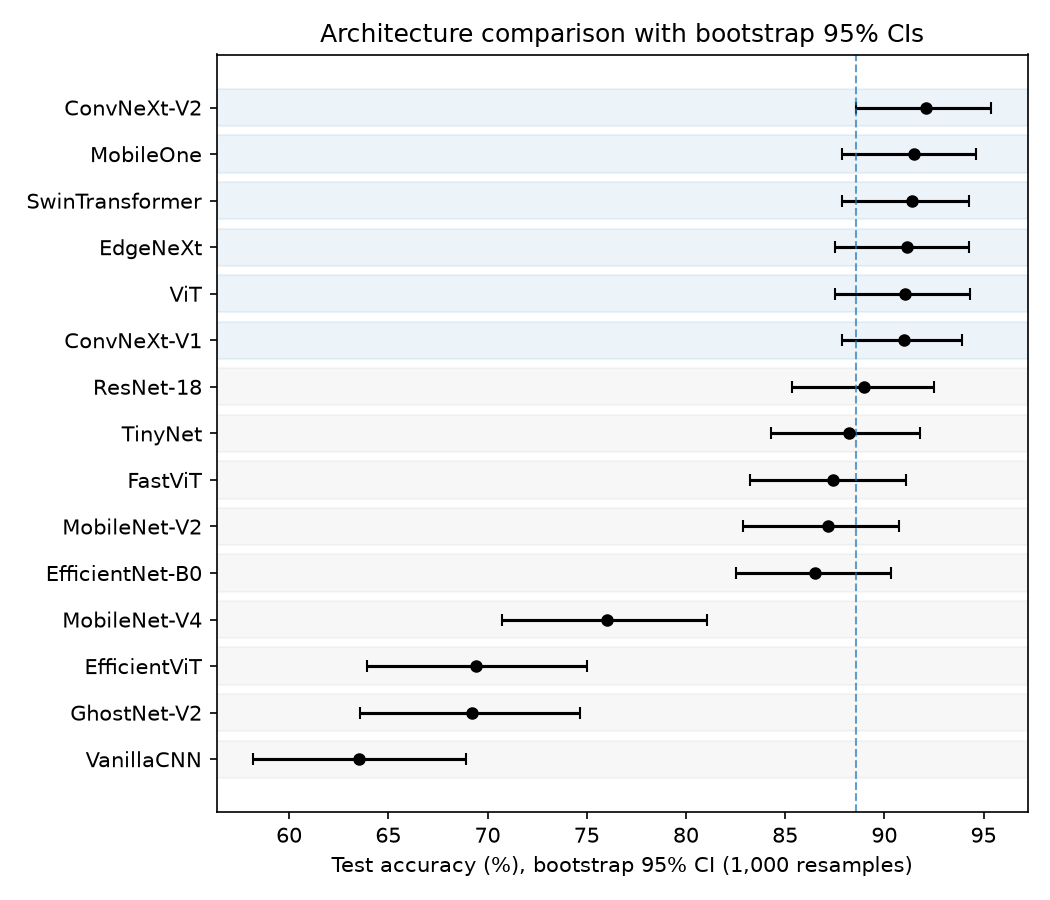
\includegraphics[width=\linewidth]{img/experiments/bootstrap/bootstrap_forest.png}
\caption{Bootstrap 95\% CI forest plot of test accuracy, sorted by point estimate. Blue rows are the six models statistically tied with ConvNeXt-V2; grey rows are significantly below it ($p<0.05$). The dashed line marks ConvNeXt-V2's lower CI bound.}
\label{fig:bootstrap_forest}
\end{figure}

\begin{table}[htbp]
\centering
\caption{Bootstrap 95\% confidence intervals (1,000 resamples) for test accuracy and macro F1 of all 15 architectures. The reported point estimates are the \emph{mean} of the 1,000 bootstrap resamples, not the single test-set value in Table~\ref{tab:arch_compare}; the two differ by at most 0.11 pp / 0.004 F1 for every model, well within the reported intervals, and the CI, not the point estimate, is what supports the statistical claims in this appendix.}
\label{tab:bootstrap_ci}
\small
\setlength{\tabcolsep}{4pt}
\begin{tabular}{lcc}
\toprule
\textbf{Model} & \textbf{Accuracy (\%) [95\% CI]} & \textbf{Macro F1 [95\% CI]} \\
\midrule
ConvNeXt-V2     & 92.11 [88.57, 95.36] & 0.898 [0.853, 0.940] \\
MobileOne       & 91.49 [87.86, 94.64] & 0.892 [0.847, 0.931] \\
SwinTransformer & 91.39 [87.86, 94.29] & 0.898 [0.855, 0.934] \\
EdgeNeXt        & 91.13 [87.50, 94.29] & 0.876 [0.827, 0.919] \\
ViT             & 91.06 [87.50, 94.29] & 0.903 [0.864, 0.940] \\
ConvNeXt-V1     & 90.98 [87.85, 93.94] & 0.893 [0.850, 0.930] \\
ResNet-18       & 88.98 [85.36, 92.50] & 0.862 [0.817, 0.908] \\
TinyNet         & 88.19 [84.29, 91.79] & 0.862 [0.815, 0.904] \\
FastViT         & 87.40 [83.21, 91.07] & 0.850 [0.801, 0.895] \\
MobileNet-V2    & 87.15 [82.86, 90.71] & 0.845 [0.794, 0.891] \\
EfficientNet-B0 & 86.52 [82.50, 90.36] & 0.836 [0.780, 0.884] \\
MobileNet-V4    & 76.03 [70.71, 81.07] & 0.720 [0.656, 0.777] \\
EfficientViT    & 69.40 [63.93, 75.00] & 0.648 [0.583, 0.714] \\
GhostNet-V2     & 69.20 [63.57, 74.64] & 0.567 [0.497, 0.640] \\
VanillaCNN      & 63.51 [58.21, 68.94] & 0.619 [0.554, 0.681] \\
\bottomrule
\end{tabular}
\end{table}

\begin{table}[htbp]
\centering
\caption{Paired bootstrap comparison of ConvNeXt-V2 against every other architecture (accuracy difference, 1,000 resamples).}
\label{tab:bootstrap_pairwise}
\small
\setlength{\tabcolsep}{4pt}
\begin{tabular}{lccc}
\toprule
\textbf{Comparison (ConvNeXt-V2 $-$ X)} & \textbf{Diff (pp)} & \textbf{95\% CI (pp)} & \textbf{$p$} \\
\midrule
SwinTransformer  & +0.68  & [$-$2.50, +3.93]   & 0.768 \\
MobileOne        & +0.72  & [$-$2.50, +3.93]   & 0.722 \\
ViT              & +1.06  & [$-$2.14, +4.29]   & 0.570 \\
EdgeNeXt         & +1.13  & [$-$2.14, +4.29]   & 0.564 \\
ConvNeXt-V1      & +1.13  & [$-$1.79, +3.93]   & 0.526 \\
ResNet-18        & +3.20  & [+0.36, +6.07]     & 0.030 \\
TinyNet          & +4.00  & [+0.36, +7.50]     & 0.034 \\
FastViT          & +4.60  & [+1.07, +8.57]     & 0.014 \\
MobileNet-V2     & +5.09  & [+1.79, +8.21]     & 0.002 \\
EfficientNet-B0  & +5.68  & [+1.79, +10.00]    & 0.002 \\
MobileNet-V4     & +16.14 & [+11.42, +21.07]   & $<$0.001 \\
GhostNet-V2      & +22.73 & [+17.14, +28.21]   & $<$0.001 \\
EfficientViT     & +22.91 & [+17.50, +28.21]   & $<$0.001 \\
VanillaCNN       & +28.64 & [+23.21, +34.29]   & $<$0.001 \\
\bottomrule
\end{tabular}
\end{table}

\textbf{Interpretation.} ConvNeXt-V2's accuracy advantage over the next five models on the leaderboard (SwinTransformer, MobileOne, ViT, EdgeNeXt, ConvNeXt-V1) is \emph{not} statistically significant at the 280-image test set size ($p > 0.5$ in all five cases; 95\% CIs on the difference all include zero). ConvNeXt-V2 is significantly more accurate than every model ranked sixth or lower ($p < 0.05$). This means the ranking of the top six models by point-estimate accuracy alone should not be over-interpreted as a strict ordering; the top six are statistically indistinguishable in accuracy on this test set. ConvNeXt-V2 remains the preferred choice not because it is proven to be the single most accurate architecture, but because among this statistically-tied top group, it has by far the smallest parameter count (3.4M against 4.3 to 85.8M for the other five) and the lowest inference latency, which is what Section~\ref{sec:experiments}'s efficiency analysis and edge-deployment motivation are based on.

\subsection{Ablation Study Significance Testing}
\label{app:bootstrap_ablation}

The same methodology is applied to the four-configuration ablation of Section~\ref{subsec:ablation}, using the per-sample predictions of each of the four BoVien checkpoints on the same 280-image test set.

\begin{table}[htbp]
\centering
\caption{Bootstrap 95\% confidence intervals (1,000 resamples) for the ablation study's four configurations.}
\label{tab:ablation_bootstrap_ci}
\small
\setlength{\tabcolsep}{4pt}
\begin{tabular}{lcc}
\toprule
\textbf{Configuration} & \textbf{Accuracy (\%) [95\% CI]} & \textbf{Macro F1 [95\% CI]} \\
\midrule
No augmentation, no class-weight & 92.11 [88.93, 95.00] & 0.898 [0.855, 0.935] \\
Augmentation, class-weighted     & 91.47 [88.21, 94.29] & 0.894 [0.849, 0.933] \\
No augmentation, class-weighted  & 90.70 [86.79, 94.29] & 0.886 [0.837, 0.928] \\
Augmentation, no class-weight    & 88.99 [85.00, 92.50] & 0.863 [0.815, 0.907] \\
\bottomrule
\end{tabular}
\end{table}

\begin{table}[htbp]
\centering
\caption{Paired bootstrap comparison of the best ablation configuration (no augmentation, no class-weight) against the other three (accuracy difference, 1,000 resamples).}
\label{tab:ablation_bootstrap_pairwise}
\small
\setlength{\tabcolsep}{4pt}
\begin{tabular}{lccc}
\toprule
\textbf{Comparison (best $-$ X)} & \textbf{Diff (pp)} & \textbf{95\% CI (pp)} & \textbf{$p$} \\
\midrule
Augmentation, class-weighted    & +0.70 & [$-$1.79, +3.21] & 0.692 \\
No augmentation, class-weighted & +1.37 & [$-$1.07, +3.93] & 0.336 \\
Augmentation, no class-weight   & +3.31 & [+0.00, +6.44]   & 0.054 \\
\bottomrule
\end{tabular}
\end{table}

\textbf{Interpretation.} None of the three pairwise differences reach the conventional $p < 0.05$ threshold at this test set size, including the largest gap (no augmentation, no class-weight, versus augmentation, no class-weight, $+$3.31pp, $p = 0.054$), whose 95\% CI lower bound sits at essentially zero. The ablation study's ranking should therefore be read as suggestive rather than conclusive. The direction is consistent (the no-augmentation configuration is the point-estimate best in three independent comparisons) and matches the sign of the discrepancy discussed in Section~\ref{sec:discussion}, but a 280-image test set and single-seed training runs cannot establish statistical significance for effects of this size (roughly 1 to 3 accuracy points). A future protocol-matched re-run with multiple random seeds per configuration, as noted in Section~\ref{sec:discussion}, would be needed to confirm the ranking rather than only its direction.

\section{LIME Faithfulness Evaluation Methodology and Per-Class Results}
\label{app:lime_faithfulness}

This appendix details the deletion-metric protocol summarised in Section~\ref{sec:experiments} (Model Interpretability) and reports the per-class breakdown.

\subsection{Protocol}

For every image in the 280-image test set, four steps are applied. (1) The model's baseline confidence in its own predicted class is recorded; (2) LIME is run with the same settings used for the qualitative examples (Quickshift segmentation, 500 perturbed samples, top 10 superpixels); (3) the superpixels LIME attributes to the predicted class are replaced with the masking colour used during LIME's own sampling (black, consistent with \texttt{hide\_color=0} in the LIME configuration), and the model is re-run on this perturbed image; (4) the confidence drop is the baseline confidence minus the perturbed-image confidence, both measured for the \emph{same} (originally predicted) class. This is the standard "deletion" faithfulness metric used in the XAI literature, in the spirit of the masking-based evaluation introduced for saliency methods by RISE \cite{petsiuk2018rise}. An explanation that faithfully identifies the pixels the model relies on should produce a large confidence drop when those pixels are removed, whereas an unfaithful or random explanation should produce a drop close to what removing a random region of the same size would cause. A 95\% confidence interval for the mean confidence drop is computed via bootstrap resampling of the 280 per-image drops (1,000 resamples, percentile method), identical in spirit to the procedure in \ref{app:bootstrap}.

\subsection{Per-Class Results}

Table~\ref{tab:lime_per_class} breaks the mean confidence drop down by true class. The two classes with the most spatially localised, high-contrast symptoms in our annotation guideline, \textit{domla} (leaf spot) and \textit{binhthuong} (healthy, where the model instead grounds its decision in the absence of any lesion pattern), show the largest drops. \textit{repsap} (mealybug damage) shows the smallest drop, consistent with the qualitative observation in Section~\ref{sec:experiments} that its damage pattern is diffuse and stippled rather than a single contiguous lesion, making it harder for a fixed-size top-10-superpixel mask to capture all of the evidence the model uses.

\begin{table}[htbp]
\centering
\caption{Mean LIME deletion-metric confidence drop by true class (280 test images total).}
\label{tab:lime_per_class}
\small
\begin{tabular}{lccc}
\toprule
\textbf{Class} & \textbf{Mean drop} & \textbf{Std} & \textbf{n} \\
\midrule
domla       & 0.769 & 0.183 & 98 \\
binhthuong  & 0.695 & 0.216 & 53 \\
moctrang    & 0.657 & 0.207 & 30 \\
gisat       & 0.589 & 0.301 & 27 \\
chaymepla   & 0.498 & 0.247 & 47 \\
repsap      & 0.416 & 0.249 & 25 \\
\bottomrule
\end{tabular}
\end{table}


\section{LLM/VLM Integration Protocol and Results}
\label{app:llm}

This appendix details the VLM-explainer protocol summarised in Section~\ref{sec:discussion}, including a secondary analysis of whether its output can double as an automatic error-detection signal. The experiment uses ConvNeXt‑V2 as the base classifier, runs on the 140 least-confident images of the 280-image test set (top 50\% by MC-Dropout predictive entropy, as in Section~\ref{sec:experiments}'s uncertainty analysis), and uses only a small, locally-hosted, zero-API-cost model (\texttt{Qwen2-VL-2B-Instruct}), reflecting a no-budget resource constraint rather than an upper bound on what larger, paid models might achieve.

\subsection{Explanation Protocol: VLM as Explainer}

The vision-language model is given the CNN's already-decided prediction, the raw image, and the LIME overlay image (boundary-marked highlighted region), and is asked only to output a boolean \texttt{supports\_cnn\_diagnosis} judgement plus free-text visual evidence, never a competing class label; the CNN's decision is never overridden. \texttt{final\_pred} is hard-set to the CNN's prediction for every image in this design (verified to hold for 100\% of rows). Of the 140 escalated images, 125 yielded a valid, parseable \texttt{supports\_cnn\_diagnosis} boolean; the remaining 15 are excluded from the scoring below since neither flag can be scored without a VLM output to compare against. We then treat \texttt{supports\_cnn\_diagnosis = False} as a zero-cost-to-CNN ``the CNN might be wrong'' flag and score it against the CNN's actual (test-set-label-derived) correctness, comparing it to a free baseline that flags the top half of this same 125-image scored subset by predictive entropy, so that both flags are evaluated on an identical denominator.

\begin{table}[htbp]
\centering
\caption{VLM disagreement flag vs. a free entropy-threshold baseline, scored against actual CNN mistakes on the 125-image subset of the 140 escalated images that yielded a parseable VLM output (19 were actual CNN mistakes).}
\label{tab:llm_flagging}
\small
\begin{tabular}{lccc}
\toprule
\textbf{Flag} & \textbf{Precision} & \textbf{Recall} & \textbf{F1} \\
\midrule
VLM (\texttt{supports\_cnn\_diagnosis = False}) & 0.40 & 0.21 & 0.28 \\
Entropy threshold (top half, free)              & 0.24 & 0.79 & 0.37 \\
\bottomrule
\end{tabular}
\end{table}

The VLM flag reaches higher precision but much lower recall than the free entropy baseline, and critically, all 4 CNN mistakes the VLM flag caught were also caught by the entropy baseline (0 complementary detections out of 19 actual mistakes); that is, the VLM's grounded, image-based explanation added no error-detection information beyond what the CNN's own predictive entropy already provides at no extra inference cost. Qualitative inspection of the generated explanations also found instances of unfaithful reasoning, e.g. one case where the VLM justified a \emph{correct} \textit{binhthuong} (healthy) prediction by describing rust-coloured spots, the symptom description belonging to a different class (\textit{gisat}), rather than reasoning from what was actually visible, underscoring that the free-text explanations should not be taken as reliably faithful without further validation.